% Trechos para colar no Overleaf da II Unidade.
% Não compilam sozinhos: copiar só o bloco que a seção pedir.

% ---------------------------------------------------------------------------
% 1) Tabela de RNF — substituir a linha do RNF-002 (hoje: 8 s)
%    Alinha com application.yml (gemini.timeout-segundos: 90) e GeminiClient
%    (até 3 tentativas se o Google devolver HTTP 503).
% ---------------------------------------------------------------------------

RNF-002 & Tempo de resposta da IA &
Até 90\,s por chamada a \texttt{generateContent}, com até 3 tentativas em caso de HTTP 503 ou falha de rede.
O valor fica em \texttt{gemini.timeout-segundos}.
A meta de 8\,s da I Unidade foi revista na implementação (o provedor não atende esse prazo de forma estável). \\

% Parágrafo para a seção 14 (se ainda estiver só ``configurado em gemini.timeout-segundos''):

O tempo da IA está definido em \texttt{gemini.timeout-segundos} (90\,s).
Se a API do Gemini responder 503 (alta demanda), o servidor tenta de novo até três vezes, com espera crescente, sem enviar nome ou e-mail do viajante.

% ---------------------------------------------------------------------------
% 2) Legendas das figuras de tela (item 13)
%    Arquivos em docs/prints/ no GitHub (branch Front-end).
%    Trocar sobretudo a lista de viagens (sem ``pitoca'') e o alerta de 80\%.
% ---------------------------------------------------------------------------

\begin{figure}[H]
\centering
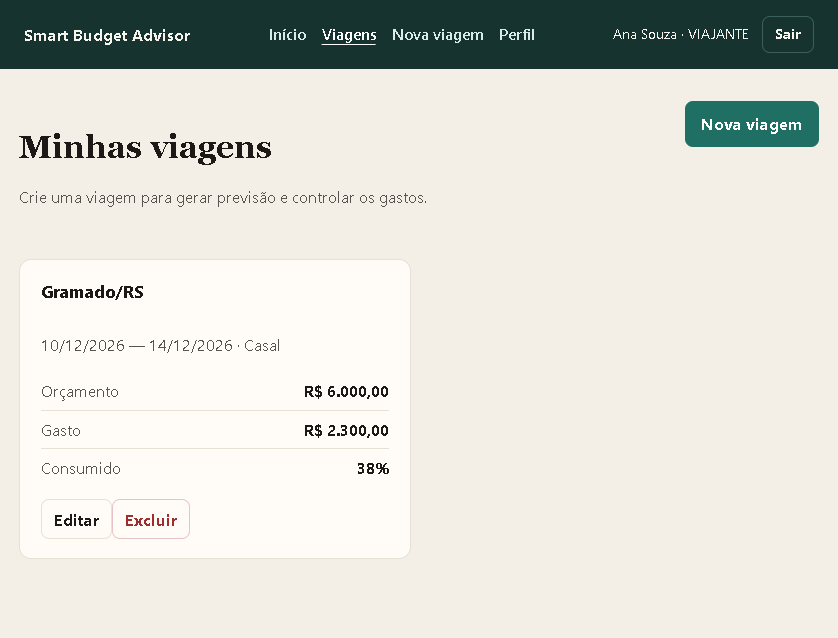
\includegraphics[width=0.92\textwidth]{prints/05-viagens.png}
\caption{Lista de viagens (RF-003). Conta demo \texttt{ana@demo.com}; apenas a viagem Gramado/RS.}
\label{fig:tela-viagens}
\end{figure}

\begin{figure}[H]
\centering
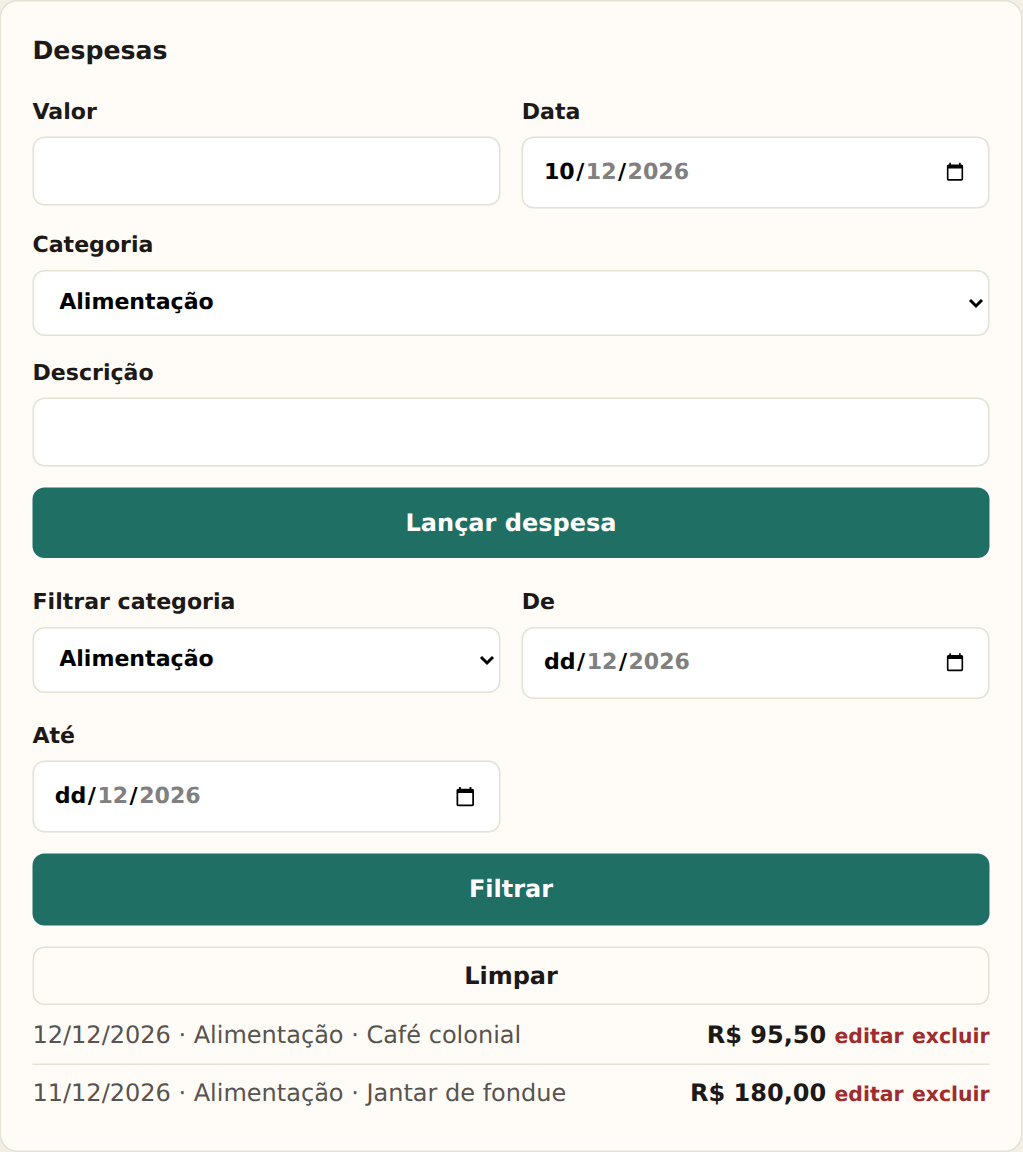
\includegraphics[width=0.92\textwidth]{prints/08e-filtro-despesas.png}
\caption{Despesas com filtro e alerta de 80\% (RF-006 e RF-007). O aviso de atenção exibe ``80\% usado'', não um valor em reais zerado. O excedente de 100\% aparece como ``+ R\$ x''.}
\label{fig:tela-alertas}
\end{figure}

% ---------------------------------------------------------------------------
% 3) Tabela de telas (se a liderança quiser atualizar a que já está no PDF)
% ---------------------------------------------------------------------------

\begin{tabular}{llp{7.2cm}}
\hline
Figura & RF & Tela \\
\hline
01-login & RF-001 & Login \\
02-cadastro & RF-001 & Cadastro com consentimento LGPD \\
03-inicio & --- & Início e status da API, banco e IA \\
04-perfil & RF-002 & Perfil, estilo e viagens anteriores \\
05-viagens & RF-003 & Lista (somente Gramado/RS) \\
06-nova-viagem & RF-003 & Criar viagem \\
07-editar-viagem & RF-003 & Editar viagem \\
08-viagem-detalhe & RF-003 & Resumo da viagem \\
08b-previsao & RF-004 & Previsão mín./recomendado/máximo \\
08c-orcamento & RF-005 & Divisão em seis categorias \\
08d-despesas & RF-006 & Lançar despesa \\
08e-filtro-despesas & RF-006, RF-007 & Filtro, editar/excluir, alerta 80\% usado \\
08f-relatorio-chat & RF-008, RF-010 & Chat da viagem e relatório \\
09-admin & --- & Painel administrativo \\
\hline
\end{tabular}

% Precisa de \usepackage{float} se usar [H]. Ajuste o \graphicspath para a pasta
% onde vocês subirem os PNG no Overleaf (ex.: \graphicspath{{prints/}{imagens/}}).
